\documentclass[conference]{IEEEtran}
\IEEEoverridecommandlockouts
\usepackage[nocompress]{cite}
\usepackage{amsmath,amssymb,amsfonts}
\usepackage{graphicx}
\usepackage{textcomp}
\usepackage{booktabs}
\usepackage{url}

\begin{document}

\title{Levels Agree, Changes Do Not: Built-Up Growth in Bujumbura, 2016 to 2025, from Three Open Products}

\author{
\IEEEauthorblockN{Kana Am\'ed\'ee}
\IEEEauthorblockA{Independent Researcher \\
Bujumbura, Burundi \\
kanaamedee00@gmail.com \\
ORCID 0009-0009-9620-6399 \\
Code: github.com/kanaamedee11/bujumbura-urban-growth-open-products}
}

\maketitle

\par\noindent{\small\bfseries\itshape Abstract. }{\small\bfseries Free global products now make it easy to ask how fast a city is growing, but they have rarely been checked against each other where ground data are scarce. We map built-up growth in Bujumbura, Burundi, from 2016 to 2025 using Dynamic World dry-season composites on Google Earth Engine, and compare it with ESA WorldCover (2020, 2021), the GHSL built-up surface (2000, 2015, 2020) and WorldPop population (2015, 2020), with SRTM terrain. Built-up levels agree well across products (correlation 0.87 to 0.88 on a 100\,m grid), but their totals for about 2020 range from 47 to 82\,km$^2$, and changes agree poorly: the correlation between Dynamic World and GHSL change is 0.17 at 100\,m and 0.36 at 1\,km, and WorldPop population change is unrelated to either (correlation 0.05 to 0.11). Dynamic World gives 25.7\,km$^2$ of newly built land between 2016 to 2018 and 2023 to 2025 (spatial-bootstrap interval 21 to 30\,km$^2$) against 5.0\,km$^2$ in GHSL over 2015 to 2020; WorldCover cannot be used for change because its two releases differ by 14\,km$^2$ in a single year. Growth is mostly infill and edge expansion: 52\% of new area lies within 100\,m of earlier built-up land and 0.6\% beyond 1\,km. New building is over-represented on slopes of 15$^\circ$ or more (7.3\% of new area against 2.5\% of earlier built-up; difference 4.8 points, interval 2.7 to 7.3) but not on the low plain below 790\,m. We conclude that the size of urban growth here depends more on the product than on the city, and give the checks needed before such numbers are used. There are no ground labels, so we cannot say which product is closest to the truth.\par}
\vspace{0.6\baselineskip}
\par\noindent{\small\bfseries\itshape Keywords. }{\small\bfseries Urban growth, built-up mapping, Dynamic World, GHSL, WorldCover, WorldPop, Bujumbura, Burundi\par}

\section{Introduction}

Bujumbura sits between Lake Tanganyika and steep hills, so where the city can grow is limited by terrain. Planners and researchers who want to know how fast it grows, and in which direction, have little to rely on besides global gridded products, because local building footprints and recent censuses are hard to obtain. Several such products are free: Dynamic World gives near real-time 10\,m land-cover probabilities from Sentinel-2 \cite{brown2022dw}; ESA WorldCover provides yearly 10\,m maps \cite{zanaga2021wc,zanaga2022wc}; the GHSL provides built-up surface at 100\,m for fixed epochs \cite{pesaresi2023ghsl}; and WorldPop provides modelled population \cite{tatem2017worldpop}.

These products are usually used one at a time. Each is validated by its authors on global samples, and a user in a small city has no way to know whether the product is accurate there, or whether two products would give the same answer. Accuracy assessment of land-cover change is known to be harder than assessment of a single map \cite{olofsson2014good,stehman2019key}, and errors that are small in a static map can be large relative to change.

This paper asks three plain questions for Bujumbura. (1) How much built-up land is there, and how much did it grow from 2016 to 2025, according to Dynamic World? (2) Do the other open products agree, on levels and on changes? (3) Where does the growth go, in terms of slope, elevation and distance from existing development? We do not train a new classifier: there are no building labels for the city, and a new model without labels would add another unchecked product. The contributions are:
\begin{enumerate}
\item \textbf{A cross-product check at city scale.} Levels agree, totals differ by a factor of 1.7, and changes agree poorly (Section~\ref{sec:agree}).
\item \textbf{A change estimate with an explicit noise floor.} Composites of three years, a placebo comparison, and a spatial block bootstrap (Section~\ref{sec:growth}).
\item \textbf{A terrain and distance analysis of new growth.} Growth is mostly infill, and over-represented on steep land (Section~\ref{sec:where}).
\item \textbf{A reproducible pipeline.} One Earth Engine script and one analysis script reproduce all numbers and figures.
\end{enumerate}
No field data or ground labels are used, so every statement is about agreement between products and not about truth.

\section{Data and Methods}

\subsection{Study area and data}
The study area is a box of 24.6\,km by 26.6\,km around Bujumbura (29.28 to 29.50$^\circ$E, 3.28 to 3.52$^\circ$S), reprojected to UTM zone 35S at 20\,m. Water is masked using the water class of both WorldCover releases, which leaves 527\,km$^2$ of land. All data were exported from Google Earth Engine \cite{gorelick2017gee}:
\begin{itemize}
\item \textbf{Dynamic World} \cite{brown2022dw}, the per-pixel ``built'' probability, taken as the median over June to September of each year from 2016 to 2025 (dry season, to limit cloud), scaled 0 to 100, with the number of observations per pixel and year.
\item \textbf{ESA WorldCover} 2020 (v100) and 2021 (v200) \cite{zanaga2021wc,zanaga2022wc}, built-up class.
\item \textbf{GHSL GHS-BUILT-S} R2023A \cite{pesaresi2023ghsl} for 2000, 2015 and 2020 at 100\,m (built surface in m$^2$ per cell).
\item \textbf{WorldPop} 100\,m population for Burundi, 2015 and 2020 \cite{tatem2017worldpop}.
\item \textbf{SRTM} 30\,m elevation and slope \cite{farr2007srtm}.
\item \textbf{Sentinel-2} \cite{drusch2012s2} true-colour dry-season median composites for 2017 and 2025, for display only.
\end{itemize}
Dynamic World is itself a Sentinel-2 product, so the true-colour images are not independent of it and are not used as evidence.

\subsection{Built-up mask and composites}
A single year of Dynamic World is noisy (Section~\ref{sec:growth}). We therefore build three-year composites as the mean of yearly built probability over years with at least three observations: early (2016 to 2018), middle (2019 to 2021) and late (2023 to 2025). A pixel is built if its composite probability is at least $\tau$. We choose $\tau$ by comparing the 2019 to 2021 composite with WorldCover 2020 (Table~\ref{tab:cal}) and use $\tau=70$, which gives the best F1 score. This makes the agreement with WorldCover at $\tau=70$ partly circular, so we do not use it as evidence of accuracy, and report results at $\tau=50$ as sensitivity. Newly built (``gain'') pixels are land that is below $\tau$ in the early composite and at or above it in the late one; ``loss'' is the reverse.

\subsection{Comparison, terrain and uncertainty}
To compare with GHSL and WorldPop, built masks are averaged onto the 100\,m grid as built fractions, keeping cells that are at least half land. Change agreement is measured as Pearson correlation of per-cell change, at 100\,m and after summing to 500\,m and 1\,km blocks. For the DW change we use 2016 to 2017 versus 2020 to 2021 to match the GHSL and WorldPop epochs as closely as the data allow.

Terrain statistics are conditional on opportunity: for each slope, elevation or distance class we report the share of land that was not built in the early composite and became built by the late one. Distance is Euclidean from the early built mask. Two uncertainty devices are used. First, a placebo change compares 2023 with the 2024 to 2025 composite, where little real change is expected; it measures the noise in the gain and loss statistics, although with a different composite depth. Second, we resample $1\times1$\,km blocks with replacement (2{,}000 draws) to give intervals for areas and for the differences between the terrain profile of new and earlier built-up land. These intervals account for sampling across space only, not for classification error.

\section{Results}

\subsection{Calibration and the annual series}
\label{sec:growth}
\begin{table}[t]
\centering
\caption{Dynamic World 2019 to 2021 composite against WorldCover 2020 built class, by threshold $\tau$. No pixel reaches $\tau=80$.}
\label{tab:cal}
\begin{tabular}{rrrrr}
\toprule
$\tau$ & DW (km$^2$) & Precision & Recall & F1 \\
\midrule
30 & 163.6 & 0.40 & 0.97 & 0.57 \\
40 & 139.7 & 0.46 & 0.96 & 0.63 \\
50 & 119.4 & 0.54 & 0.95 & 0.69 \\
60 & 100.3 & 0.62 & 0.93 & 0.75 \\
70 & 73.7 & 0.77 & 0.85 & 0.81 \\
\bottomrule
\end{tabular}
\end{table}
At low thresholds Dynamic World marks far more land as built than WorldCover (164\,km$^2$ against 67\,km$^2$), with high recall and low precision. Even at $\tau=70$ the totals differ (74 against 67\,km$^2$).

\begin{figure}[t]
\centering
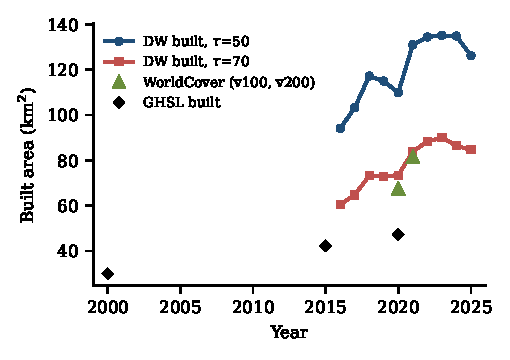
\includegraphics[width=\columnwidth]{figures/fig_series.pdf}
\caption{Built-up area in the study box. Dynamic World yearly series (two thresholds) is noisy; the three other products give very different totals for about 2020.}
\label{fig:series}
\end{figure}
Figure~\ref{fig:series} shows that yearly Dynamic World built area at $\tau=70$ rises from 60.5\,km$^2$ in 2016 to 84.6\,km$^2$ in 2025, but not smoothly: it peaks at 90.0\,km$^2$ in 2023, and at $\tau=50$ the 2016 to 2025 series (94 to 126\,km$^2$) falls by 9\,km$^2$ between 2023 and 2025 and by 7\,km$^2$ between 2018 and 2020. The median number of clear observations per pixel ranges from 5 to 16 per season (16 in 2016, 5 in 2023), so year-to-year steps partly reflect sampling. Single-year differences should not be read as growth.

\subsection{Size and shape of growth}
With three-year composites at $\tau=70$, built area rises from 62.6\,km$^2$ (2016 to 2018) to 83.9\,km$^2$ (2023 to 2025), a gain of 25.7\,km$^2$ and a loss of 4.4\,km$^2$ (net $+21.3$\,km$^2$, $+34\%$). At $\tau=50$ the gain is 34.2\,km$^2$ and the loss 5.6\,km$^2$. The block bootstrap gives 21 to 30\,km$^2$ for the gain at $\tau=70$. The placebo comparison gives 2.8\,km$^2$ of gain, about a tenth of the measured value, but 9.6\,km$^2$ of loss, more than twice the measured loss, so the loss is not distinguishable from noise and we do not interpret it. Of the 25.7\,km$^2$ of gain, 11.3\,km$^2$ (44\%) is also built in WorldCover 2021. The rest is not confirmed by that product, and the two are separated by up to four years.

Gain is made of 2{,}257 connected patches; 241 patches of at least 1\,ha make up 22.8\,km$^2$ (88\%), and the largest is 3.1\,km$^2$ (Fig.~\ref{fig:maps}). Growth is therefore a small number of large developments plus many small additions.

\begin{figure*}[t]
\centering
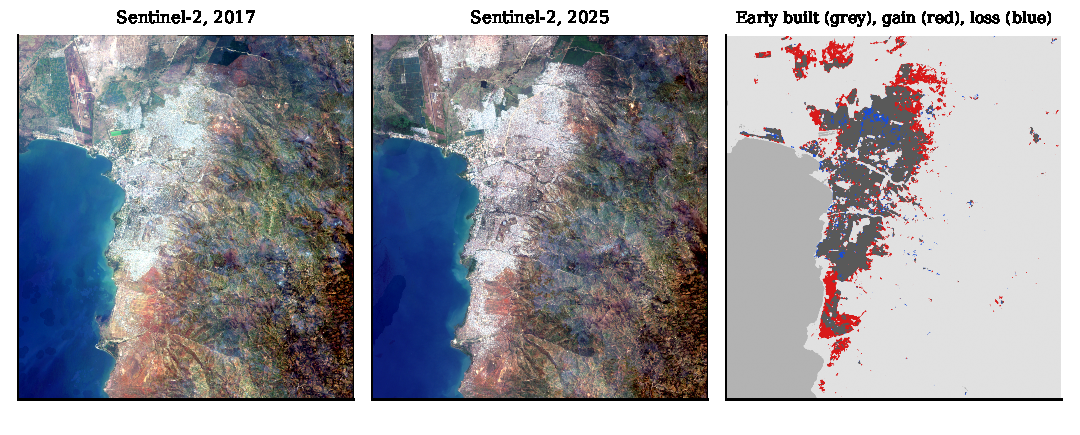
\includegraphics[width=\textwidth]{figures/fig_maps.pdf}
\caption{Sentinel-2 dry-season composites for 2017 and 2025 (left, middle) and the built-up change map (right): earlier built-up (grey), gain (red), loss (blue), $\tau=70$. Lake Tanganyika lies to the west.}
\label{fig:maps}
\end{figure*}

\subsection{Agreement between products}
\label{sec:agree}
For about 2020 the products give different built-up areas: GHSL 47.3\,km$^2$ (land cells of the box), Dynamic World 73.7\,km$^2$ ($\tau=70$), WorldCover v100 67.4\,km$^2$ and WorldCover v200 81.5\,km$^2$, a spread of 1.7 times. WorldCover itself increases by 14.1\,km$^2$ from its 2020 to its 2021 release, which is a change of release, not of the city; we therefore do not use it for change.

\begin{figure}[t]
\centering
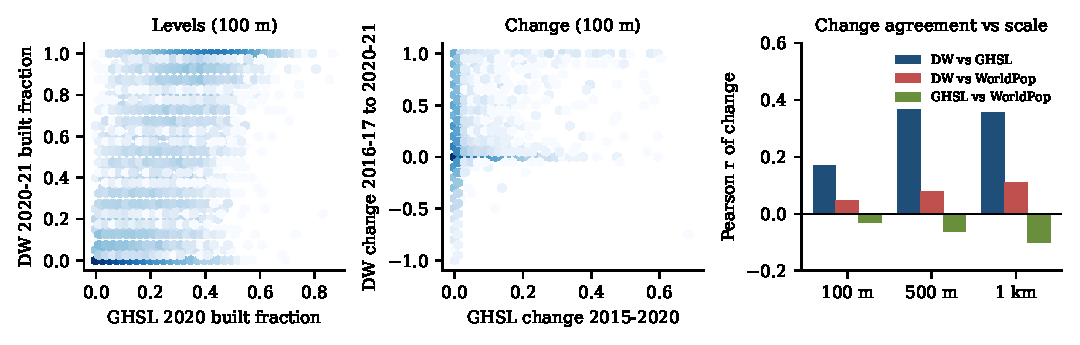
\includegraphics[width=\columnwidth]{figures/fig_agree.pdf}
\caption{Agreement on a 100\,m grid. Left: built fraction in 2020 (GHSL) against Dynamic World. Middle: change in each product. Right: correlation of change after aggregation to coarser blocks.}
\label{fig:agree}
\end{figure}
On the 100\,m grid the built fractions of Dynamic World and GHSL correlate at 0.88 in 2020 and 0.87 in 2015 (Fig.~\ref{fig:agree}, left). Their changes do not: the correlation is 0.17 at 100\,m, and rises only to 0.37 at 500\,m and 0.36 at 1\,km. In total, Dynamic World gains 15.7\,km$^2$ between 2016 to 2017 and 2020 to 2021 on the common grid, and GHSL gains 5.0\,km$^2$ from 2015 to 2020. WorldPop's population change is nearly unrelated to the built-up change in either product (0.05 to 0.11 with Dynamic World, $-0.03$ to $-0.10$ with GHSL, across the three scales).

\subsection{Population}
In the land cells of the box, WorldPop rises from 895{,}000 to 1{,}108{,}000 people between 2015 and 2020 (+24\%), while GHSL built surface rises by 12\%, so built surface per person falls from 47 to 43\,m$^2$. Of the added population, 29\% falls in 100\,m cells that were less than 10\% built in 2015. WorldPop is a modelled product, and its 2015 and 2020 surfaces are not guaranteed to be independent estimates of change, so we treat this only as a description of the products. We did not test why change in WorldPop is uncorrelated with built-up change.

\subsection{Where growth goes}
\label{sec:where}
\begin{figure*}[t]
\centering
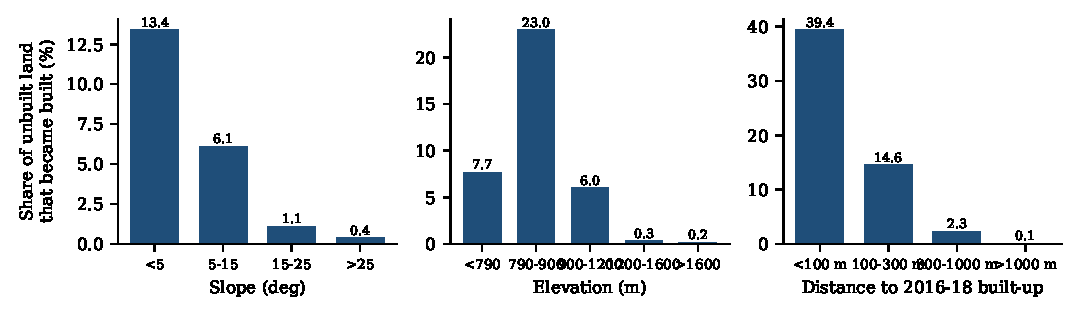
\includegraphics[width=\textwidth]{figures/fig_terrain.pdf}
\caption{Share of land unbuilt in 2016 to 2018 that became built by 2023 to 2025, by slope, elevation and distance from early built-up land ($\tau=70$).}
\label{fig:terrain}
\end{figure*}
Growth is concentrated near existing development (Fig.~\ref{fig:terrain}, right). Of previously unbuilt land within 100\,m of the early built mask, 39\% became built; within 100 to 300\,m, 15\%; 300 to 1000\,m, 2.3\%; beyond 1\,km, 0.07\%. By area, 52\% of the gain lies within 100\,m of earlier built-up land, 85\% within 300\,m, and only 0.6\% beyond 1\,km, so leapfrog development is negligible in this record.

Slope matters in the expected direction: 13\% of unbuilt land below 5$^\circ$ became built, 6.1\% at 5 to 15$^\circ$, 1.1\% at 15 to 25$^\circ$ and 0.4\% above 25$^\circ$. The highest rate by elevation is in the 790 to 900\,m band (23\%), the foothill strip just above the plain, against 7.7\% below 790\,m.

\begin{table}[t]
\centering
\caption{Terrain profile of earlier built-up land and of new gain ($\tau=70$). Intervals are 95\% block-bootstrap intervals (sampling over space only).}
\label{tab:exp}
\scriptsize\setlength{\tabcolsep}{2pt}\begin{tabular}{lccc}
\toprule
 & Earlier & Gain & Diff. \\
\midrule
Slope $\geq 15^\circ$ (\%) & 2.5 [1.6, 3.5] & 7.3 [4.8, 10.4] & $+4.8$ [2.7, 7.3] \\
Below 790\,m (\%) & 20.9 [14.7, 28.2] & 20.1 [14.3, 26.5] & $-0.8$ [$-8.0$, 6.4] \\
\bottomrule
\end{tabular}
\end{table}
New building is over-represented on steep land (Table~\ref{tab:exp}): 7.3\% of new area is on slopes of 15$^\circ$ or more (1.9\,km$^2$), against 2.5\% of earlier built-up land, although 43\% of all land in the box is that steep. New building is not over-represented on the low plain below 790\,m: the share is about 20\% in both groups, with an interval that includes zero (5.2\,km$^2$ of gain). We use 790\,m as a convenient cut for the lake plain and have not tied it to any flood level. SRTM has metre-scale vertical error, and we did not map flood exposure.

\section{Discussion and Limitations}

The main finding is about the products. Three open sources agree that Bujumbura has a large built core and that it grew, but they disagree by a factor of 1.7 on how much land is built, by a factor of 3 on how much was added, and almost entirely on where it was added. A user who picks one product gets an answer that depends mostly on that choice. We do not know which is closest to the truth. Dynamic World is a probability from a deep model that was not designed for change, GHSL is built from Sentinel-2 and Landsat composites with fixed epochs, and the products do not define ``built'' identically (for example, in how they treat roads, bare compacted soil and informal housing).

Limits of this study are as follows. (i) There are no ground labels, so no accuracy is reported. (ii) $\tau$ was chosen against WorldCover 2020, and the gain depends on it (25.7\,km$^2$ at 70, 34.2\,km$^2$ at 50). (iii) Gain and loss are defined by threshold crossing, so some of both is noise: the placebo comparison suggests that for gain it is small (about a tenth), but for loss it is as large as the signal. (iv) Observation counts differ between years. (v) Bootstrap intervals reflect spatial sampling only. (vi) Product epochs differ (2015, 2020, 2021 versus our composites), which lowers apparent agreement of change. (vii) One city, one season definition and one threshold rule.

A fair test would use a sample of building footprints or very-high-resolution imagery, labelled by someone who knows the city, to estimate each product's error for change. Open building footprints for Bujumbura, if available, would be the first source to try.

\section{Conclusion}

For Bujumbura, three widely used open products agree on where the city is but not on how much it has grown or whether it has grown where people have settled. Dynamic World shows 25.7\,km$^2$ of gain (21\,km$^2$ net of loss) between 2016 to 2018 and 2023 to 2025, mostly infill and edge expansion within 300\,m of existing development, with a small but statistically clear excess on steep land. GHSL shows a fraction of that, WorldCover cannot be used for change, and WorldPop change is unrelated to built-up change. Users of these products for planning should not trust a single source, should report change with a placebo estimate of its noise, and should check at least a few hundred locations on the ground or on very-high-resolution imagery.

\bibliographystyle{IEEEtran}
\bibliography{references}

\end{document}
